\documentclass[10pt,a4paper]{article}
\usepackage[margin=1.7cm,top=1.2cm,bottom=1.0cm]{geometry}
\usepackage{booktabs,array,xcolor,amsmath}
\usepackage{tikz}
\usetikzlibrary{arrows.meta,calc}
\pagestyle{empty}
\setlength{\parindent}{0pt}
\setlength{\parskip}{4pt}

\definecolor{good}{HTML}{1B7F4B}
\definecolor{bad}{HTML}{B3261E}
\definecolor{vox}{HTML}{3B6FB6}
\definecolor{cab}{HTML}{222222}

\newcommand{\panel}[1]{{\small\bfseries #1}}

\begin{document}

\begin{center}
{\Large\bfseries Why voxel FEM suits a sphere but not a cable}\\[2pt]
{\small PhysX volumetric deformables in Isaac Sim --- one-page note}
\end{center}

\textbf{Claim.} Isaac Sim builds the FEM simulation mesh from \emph{cubic voxels}
of one size, $h = L_{\max}/N$, where $L_{\max}$ is the body's longest dimension and
$N$ the hexahedral resolution. The number of voxels across the \emph{thinnest}
dimension $d$ is therefore $n_\perp = N\,d/L_{\max}$.
A sphere has $d/L_{\max}=1$; our cable has $d/L_{\max}=1/223$, so its cross-section
--- the only thing that sets bending stiffness --- is left unresolved.

\vspace{2pt}
% ---------------------------------------------------------------- row 1
\begin{minipage}[t]{0.30\linewidth}
\centering
\panel{\textcolor{good}{Sphere, $N=10$}}\\[3pt]
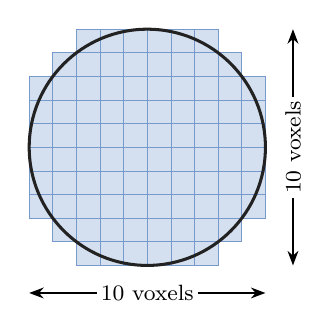
\begin{tikzpicture}[x=1cm,y=1cm]
  \foreach \i in {0,...,9}{\foreach \j in {0,...,9}{
    \pgfmathsetmacro\cx{(\i+0.5)*0.3-1.5}
    \pgfmathsetmacro\cy{(\j+0.5)*0.3-1.5}
    \pgfmathtruncatemacro\inside{(max(abs(\cx)-0.15,0)^2+max(abs(\cy)-0.15,0)^2) < 2.25 ? 1 : 0}
    \ifnum\inside=1
      \fill[vox!22] (\cx-0.15,\cy-0.15) rectangle ++(0.3,0.3);
      \draw[vox!70,line width=0.3pt] (\cx-0.15,\cy-0.15) rectangle ++(0.3,0.3);
    \fi
  }}
  \draw[cab,line width=1.1pt] (0,0) circle (1.5);
  \draw[<->,>=Stealth,line width=0.5pt] (-1.5,-1.85) -- (1.5,-1.85)
    node[midway,fill=white,inner sep=1.5pt]{\footnotesize 10 voxels};
  \draw[<->,>=Stealth,line width=0.5pt] (1.85,-1.5) -- (1.85,1.5)
    node[midway,fill=white,inner sep=1.5pt,rotate=90]{\footnotesize 10 voxels};
\end{tikzpicture}\\[2pt]
{\footnotesize 10 voxels across in \emph{every} direction.\\
$\tfrac{\pi}{6}N^3 \approx 520$ voxels, isotropic.}
\end{minipage}\hfill
\begin{minipage}[t]{0.67\linewidth}
\centering
\panel{\textcolor{bad}{Cable, $N=130$}}\\[3pt]
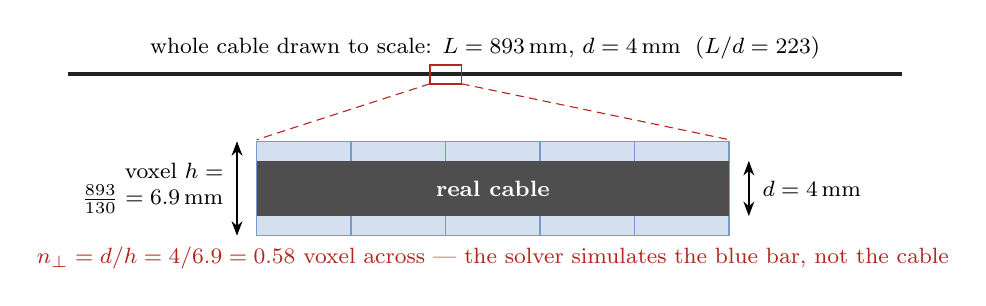
\begin{tikzpicture}[x=1cm,y=1cm]
  % the whole cable, to scale: 893 mm -> 10.6 cm, so 4 mm -> 0.47 mm
  \draw[cab,line width=1.35pt] (0,2.55) -- (10.6,2.55);
  \node[anchor=south,font=\footnotesize] at (5.3,2.62)
    {whole cable drawn to scale: $L=893$\,mm, $d=4$\,mm \;($L/d=223$)};
  \draw[bad,line width=0.6pt] (4.6,2.43) rectangle (5.0,2.67);
  \draw[bad,line width=0.4pt,densely dashed] (4.6,2.43) -- (2.4,1.72);
  \draw[bad,line width=0.4pt,densely dashed] (5.0,2.43) -- (8.4,1.72);

  % zoom: five voxels of 6.9 mm drawn 1.2 cm wide, cable 4/6.9*1.2 = 0.70 cm
  \foreach \k in {0,...,4}{
    \fill[vox!22] (2.4+1.2*\k,0.5) rectangle ++(1.2,1.2);
    \draw[vox!70,line width=0.5pt] (2.4+1.2*\k,0.5) rectangle ++(1.2,1.2);
  }
  \fill[cab!80] (2.4,0.75) rectangle (8.4,1.45);
  \node[white,font=\footnotesize\bfseries] at (5.4,1.10) {real cable};
  \draw[<->,>=Stealth,line width=0.5pt] (2.15,0.5) -- (2.15,1.7);
  \node[anchor=east,font=\footnotesize,align=right] at (2.10,1.10)
    {voxel $h=$\\$\tfrac{893}{130}=6.9$\,mm};
  \draw[<->,>=Stealth,line width=0.5pt] (8.65,0.75) -- (8.65,1.45);
  \node[anchor=west,font=\footnotesize,align=left] at (8.70,1.10)
    {$d=4$\,mm};
  \node[font=\footnotesize,text=bad] at (5.4,0.22)
    {$n_\perp = d/h = 4/6.9 = 0.58$ voxel across --- the solver simulates the blue bar, not the cable};
\end{tikzpicture}\\[2pt]
{\footnotesize One row of voxels, each \emph{larger} than the cable. A $6.9$\,mm square bar has
$I=h^4/12$, about $15\times$ the cable's $\pi r^4/4$: bending is $\sim\!15\times$ too stiff.}
\end{minipage}

\vspace{3pt}
% ---------------------------------------------------------------- row 2
\panel{The two ways out, and why neither works}
\hfill{\footnotesize (cross-sections below share one scale)}

\vspace{1pt}
\begin{center}
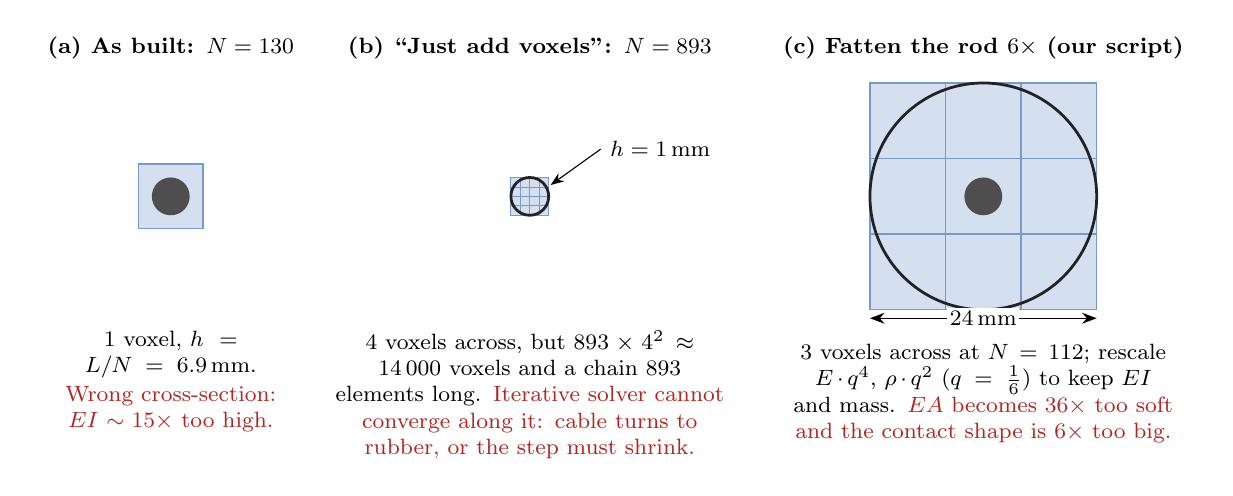
\begin{tikzpicture}[x=0.12cm,y=0.12cm]  % 1 unit = 1 mm
  % ---- (a) what we get
  \begin{scope}[shift={(14,0)}]
    \fill[vox!22] (-3.43,-3.43) rectangle (3.43,3.43);
    \draw[vox!70,line width=0.5pt] (-3.43,-3.43) rectangle (3.43,3.43);
    \fill[cab!80] (0,0) circle (2);
    \node[font=\footnotesize\bfseries,anchor=south] at (0,13.5) {(a) As built: $N=130$};
    \node[font=\footnotesize,anchor=north,text width=3.4cm,align=center] at (0,-13.2)
      {1 voxel, $h=L/N=6.9$\,mm.\\[1pt]\textcolor{bad}{Wrong cross-section: $EI$ $\sim\!15\times$ too high.}};
  \end{scope}
  % ---- (b) more voxels
  \begin{scope}[shift={(52,0)}]
    \foreach \i in {-2,...,1}{\foreach \j in {-2,...,1}{
      \fill[vox!22] (\i,\j) rectangle ++(1,1);
      \draw[vox!70,line width=0.3pt] (\i,\j) rectangle ++(1,1);
    }}
    \draw[cab,line width=1pt] (0,0) circle (2);
    \draw[->,>=Stealth,line width=0.4pt] (7.5,5) node[anchor=west,font=\footnotesize]{$h=1$\,mm} -- (2.2,1.2);
    \node[font=\footnotesize\bfseries,anchor=south] at (0,13.5) {(b) ``Just add voxels'': $N=893$};
    \node[font=\footnotesize,anchor=north,text width=5.0cm,align=center] at (0,-13.2)
      {4 voxels across, but $893\times4^2\approx 14\,000$ voxels and a chain 893 elements long.
       \textcolor{bad}{Iterative solver cannot converge along it: cable turns to rubber, or the step must shrink.}};
  \end{scope}
  % ---- (c) fat rod
  \begin{scope}[shift={(100,0)}]
    \foreach \i in {-1,...,1}{\foreach \j in {-1,...,1}{
      \fill[vox!22] (8*\i-4,8*\j-4) rectangle ++(8,8);
      \draw[vox!70,line width=0.5pt] (8*\i-4,8*\j-4) rectangle ++(8,8);
    }}
    \draw[cab,line width=1pt] (0,0) circle (12);
    \fill[cab!80] (0,0) circle (2);
    \draw[<->,>=Stealth,line width=0.5pt] (-12,-12.9) -- (12,-12.9);
    \node[font=\footnotesize,fill=white,inner sep=1pt] at (0,-12.9) {24\,mm};
    \node[font=\footnotesize\bfseries,anchor=south] at (0,13.5) {(c) Fatten the rod $6\times$ (our script)};
    \node[font=\footnotesize,anchor=north,text width=5.4cm,align=center] at (0,-14.6)
      {3 voxels across at $N=112$; rescale $E\!\cdot\!q^4$, $\rho\!\cdot\!q^2$ ($q=\tfrac16$) to keep $EI$ and mass.
       \textcolor{bad}{$EA$ becomes $36\times$ too soft and the contact shape is $6\times$ too big.}};
  \end{scope}
\end{tikzpicture}
\end{center}

\vspace{-2pt}
\panel{Calculations}

{\small
\textbf{Inputs:} $L=893$\,mm (from the photo), $r=2$\,mm, $d=4$\,mm, $E=80$\,MPa,
$\rho=2390$\,kg/m$^3$ (\texttt{cable\_config.py}); $N=130$, $r_\text{sim}=12$\,mm,
$\Delta t=1/240$\,s (\texttt{hang\_physx\_fem.py}).}

\vspace{2pt}
\renewcommand{\arraystretch}{1.25}
{\small
\begin{minipage}[t]{0.50\linewidth}
\textbf{Thin cable, $d=4$\,mm}\\[1pt]
\begin{tabular}{@{}l@{\quad}l@{}}
aspect ratio & $L/d = 893/4 = 223$ \\
voxel size & $h = L/N = 893/130 = 6.9$\,mm \\
voxels across & $n_\perp = d/h = 4/6.9 = 0.58$ \\
bending error & $\dfrac{h^4/12}{\pi r^4/4} = \dfrac{1.9\times10^{-10}}{1.3\times10^{-11}} \approx 15$ \\[6pt]
4 voxels across & $N = 4L/d = 4\cdot893/4 = 893$ \\
number of voxels & $893\cdot4^2 \approx 14\,000$ \\
wave speed & $c=\sqrt{E/\rho}=\sqrt{80\times10^{6}/2390}=183$\,m/s \\
crossing time & $h/c = 1\,\text{mm}/183 = 5.5\,\mu$s \\
step / crossing & $\Delta t/(h/c) = (1/240)/5.5\,\mu\text{s} \approx 760$ \\
\end{tabular}
\end{minipage}\hfill
\begin{minipage}[t]{0.48\linewidth}
\textbf{Fat rod, $r_\text{sim}=12$\,mm}\\[1pt]
\begin{tabular}{@{}l@{\quad}l@{}}
radius ratio & $q = r/r_\text{sim} = 2/12 = 1/6$ \\
resolution & $N=\lceil 3L/(2r_\text{sim})\rceil = 112$,\; $h = 8.0$\,mm \\
voxels across & $n_\perp = 24/8.0 = 3$ \\
rescaled material & $E q^4 = 62$\,kPa,\; $\rho q^2 = 66$\,kg/m$^3$ \\
stretch stiffness & $EA$: $1005\,\text{N} \to 28\,\text{N}$ \;($q^2 = 1/36$) \\
\end{tabular}

\vspace{3pt}
\textbf{Thick cable, $d=20$--$30$\,mm}\\[1pt]
\begin{tabular}{@{}l@{\quad}l@{}}
aspect ratio & $893/20 = 45$,\; $893/30 = 30$ \\
voxels across & $20/6.9 = 2.9$,\; $30/6.9 = 4.4$ \\
4 voxels across & $N = 4\cdot893/20 = 179$,\; $4\cdot893/30 = 120$ \\
step / crossing & $6.9\,\text{mm}/183 = 38\,\mu$s,\; ratio $\approx 110$ \\
\end{tabular}
\end{minipage}}

\vspace{3pt}
\renewcommand{\arraystretch}{1.05}
\begin{center}\footnotesize
\begin{tabular}{@{}l c c c@{}}
\toprule
 & \textbf{Sphere} & \textbf{Thin cable} ($d=4$\,mm) & \textbf{Thick cable} ($d=20$--$30$\,mm) \\
\midrule
Longest / thinnest dimension & 1 & 223 & 45--30 \\
Voxels across the thin direction at $N=130$ & 130 & 0.58 & 2.9--4.4 \\
$N$ needed for 4 voxels across & 4 & 893 & 179--120 \\
Element chain the solver must converge along & $N$ & 893 & 120--179 \\
Result & good & bad & works \\
\bottomrule
\end{tabular}
\end{center}

\vspace{1pt}
\fcolorbox{good}{good!7}{\parbox{\dimexpr\linewidth-2\fboxsep-2\fboxrule}{%
\textbf{Conclusion.} Voxel FEM fits compact bodies and thick cables, where the grid
resolves the cross-section. A thin cable is a one-dimensional object and should be
modelled as one --- a Cosserat rod or a capsule chain --- where the cross-section
enters through $EI$, $EA$ and $GJ$. The rod and capsule-chain models in this project
reproduce the photographed cable to 33--75\,mm RMS (\texttt{metrics.csv}).}}

\end{document}
